\section{Introduction}

Critical infrastructures are integral to the functioning of our daily lives. They are changing in order to solve different problems it faces nowadays. The growth of power demand, integration of markets and the need of sustainable and efficient energy sources. \\
One such important critical infrastructure is the smart grid. A typical smart grid is divided into several domains such as generation, transmission and distribution. All the actors within domains of a smart grid are connected through information and communication technology(ICT). Hence, energy grids have continuously been the target of cyber attacks and provided their use of standard architecture and internet, they are relatively easier to attack. Security mechanisms have been introduced to protect against such attacks. Security-by-design approach has been used to determine security measures for various systems during design phase. With this approach, the system is equipped to deal with difficult scenarios before deployment. \\ However, there may be instances where the operator must intervene to control the system when under attack and stress. During such instances, the user maybe asked to re-authenticate themselves, at which point remembering increasingly difficult passwords and entering it correctly actually causes an overhead on the operator. The security mechanism in fact is a hindrance here. Such a situation could be avoided if the authentication system in place is usable under different conditions. 


\section{Related Work}
Usability of security is an area of research that has been largely ignored. More focus has been placed on security itself, hence the presence of extensive literature on security in information systems and lack thereof in the case of usability. Smart grid is a vast interconnection of several different kinds of components across several domains. There are several key components that interact with each other that expose several vulnerabilities\cite{liu2012cyber}. There are several vulnerabilities across communication protocols, legacy devices and technologies. Additionally, when designing a system, new vulnerabilities may be found, rendering current security infrastructure weaker. A cyber-physical approach\cite{mo2012cyber} has been presented to tackle new security challenges. They propose a system model using security requirements and vulnerabilities to identify countermeasures. In order to identify security requirements, a concrete network architecture is required. From the architecture, security objectives can be derived and threats can be evaluated to determine the requirements for security. Wang et. al\cite{wang2013cyber} provide a comprehensive categorization and evaluation of network threats and discuss their countermeasures in detail.
\newline 
There is a lack of usability standards that determine the goals of usability for energy systems. Usability is not directly engineered, but is rather a consequence of system engineering. There are guidelines that aid engineers in developing usable systems\cite{nurse2011guidelines}. Standards such as ISO 9241-11\cite{bevan2015iso} state that usability must be measured in terms of effectiveness, efficiency and satisfaction. These terms must be related to the system of interest using performance metrics of the respective system. A first look at such a relation is provided\cite{kainda2010security}, however is not comprehensive enough to establish a concrete relation between systems. In this paper, we build on this idea to derive a usable security by design approach that begins at the design phase\cite{nielsen1992usability}. The goal of this research to establish how usability of security in power plants can be achieved. A second goal is to reduce the burden on a power plant operator, since the operation of a power plant can be stressful. We assume that the operator of the power plant is oblivious to the security design. Additionally, we assume there is an authentication system in place whose goal is to protect the system and authenticate legitimate operators and is expected to function with high efficiency. We shall focus only on security and usability and their relation. Hence, usability of other systems are not considered. Only systems having an user interface are considered.

\section{Security in Virtual Power Plants}

The availability of electric power is the primary goal of the smart grids. As the smart grid develops, these power systems are more sophisticated, using modern technology allowing better control and reliability. Smart grid will feature a highly interconnected network, opening up the possibility for new vulnerabilities.\\

%\textbf{Virtual Power Plant \& Security Issues}\\

Virtual Power Plant(VPP) is one such infrastructure. A VPP is a centralized system that aggregates various energy sources to meet the energy demand of a geographical area. It relies upon software to remotely control, optimize and dispatch energy from Distributed Energy resources(DERs). At the heart of every VPP is the Energy Management System(EMS). The EMS manages power flows in order to minimize the electricity generation costs and avoid loss of energy produced by generators based on renewable energy sources. The EMS consists of a set of software programs designed to control and monitor several aspects of the power plant such as generation levels, capacity, current and voltage levels, power fluctuations, supply-demand matching and so on. These software programs are automated and carry out operations based on pre-defined rules and functions. They are consistently monitored by an operator, known as VPP Operator. Therefore, a VPP is a system that employs software and networking tools making it susceptible to cyber attacks. There are several known ways to attack a power plant, network based attacks such as man-in-the-middle, Masquerading, Spoofing, Denial of service, Injection etc, software vulnerability based attacks, hardware based attacks and so on. Most of the known attacks have defined countermeasures which are in use to protect the power plant. Even with the presence of an extensive defense infrastructure, there may be new and unprecedented attacks on power plants, including those that exploit zero-day vulnerabilities. 
\newline
A virtual power plant under attack is expected to continue functioning normally, i.e, it must primarily meet the goal of availability to the customer end. In anticipation of such attacks, the system may be configured to reschedule, find replacement sources or even attempt to control the system to prevent its shutdown or damage. The operator may be requested to control the system in case of unprecedented events or cases where the operator's intervention or authorization are required. For example, consider a scenario when a power plant is under attack and its primary generation units are inaccessible. The VPP then attempts to find replacement units. However, in case of a large scale attack units in the neighbourhood may also be rendered inaccessible. Therefore, the VPP may have to look for units outside its allotted area which may require operator request and authorization. In such a case, the operator is required to access and operate the system. We assume there is an authentication mechanism in place that protects the system from unauthorized access, and therefore is the first interface the operator comes across. This authentication interface is vital since it prevents unauthorized personnel from accessing the system either in normal system state or when the system is under attack, which could be orchestrated by the unauthorized personnel themselves. The authentication mechanism should however be a usable mechanism, even under stress, to prevent the legitimate power plant operator from being locked out. A traditional username-password system in this case could potentially be a problem. The operator is required to recall and enter the information accurately in order to be granted access. In such a situation, the operator may find it difficult to recall a complex password and is more likely to make mistakes entering it and being denied access, which could lead to a catastrophe. 

\smallskip

Traditional authentication mechanisms are largely based on password based systems. Having a long random password is good advice. Unfortunately, when faced with having to remember several random fifteen character passwords (characters being A to Z, a to z, 0 to 9 and an assortment of other printable characters such as ! @ \# \$ and \%), most users apply a judgement to the value of the information protected by the password and act accordingly. 
Secure passwords may be constructed from a combination of alphabets, numbers and symbols. There is a trade off though, as such passwords are harder to remember and also hard to enter into a system without errors. It is also compounded by the fact that users are recommended to change passwords periodically. Users tend to create variations of their previous passwords to prevent having to generate a new password and consider using a variant of a previous password easier since they are already familiar with it. This is especially problematic since users may forget the password has been changed and do not remember the new password, inviting a lot of pressure onto users who are not technologically friendly and are oblivious to the system structure. Therefore, the most secure passwords and password systems are, in fact, the least usable. 

\smallskip

Therefore, with usability and security being a trade-off, organizations often prioritize security over usability. Hence, to bridge this gap between the two, a framework is required. A framework which can unite the two and allow a system to be secure as well as usable. In the next section, we look towards such a usable security framework. Since the focus is usability, we consider authentication mechanisms, which are security mechanisms in place that are directly interfaced by an operator. Most other security mechanisms affect software and hardware performance but do not impact usability and user performance since there is no existing interface to the security infrastructure.

\section{Usability: What is it?}

Usability is a measure of the interactive user experience associated with a user interface, such as a website or software application. A user-friendly interface design is easy-to-learn, supports users' tasks and goals efficiently and effectively, and is satisfying and engaging to use.
\newline
An interface's level of usability can be measured by inviting intended users of the system to participate in a usability testing session. During a usability test session, a user is given a series of tasks to complete by using the system in question, without any assistance from the researcher. The researcher records user behaviours, emotional reactions, and the user's performance as they attempt to accomplish each task. The researcher takes note of any moments of confusion or frustration that the user experienced while trying to complete a task and also tracks whether or not the user was able to satisfactorily complete each task. Analysis of data from several users provides User Experience Engineers a means of recommending how and where to re-design the interface in order to improve its level of usability and thus, the user experience in general.

\smallskip

Usability is the ease of use of a software by any individual in any situation to achieve certain objectives with efficiency. This software, developed by experts, must be usable by any other person effectively. Therefore, the software will have to be developed with a user-centered approach. "Ease of Use" encapsulates the following terms:

\begin{itemize}

\item Effective: Effectiveness is the completeness and accuracy with which users achieve specified goals. It is determined by looking at whether the user's goals were met successfully and whether all work is correct.

\item Efficient: Efficiency can be described as the speed (with accuracy) in which users can complete the tasks for which they use the product. ISO 9241 defines efficiency as the total resources expended in a task. Efficiency metrics include the number of clicks or keystrokes required or the total "time on task".

\item Satisfaction: The comfort and acceptability of use. Additionally, the following two are also considered,

\item Error Tolerant: The ultimate goal is a system which has no errors. But, product developers are human, and computer systems are far from perfect, so errors may occur. An error tolerant program is designed to prevent errors caused by the user's interaction and to help the user in recovering from any errors that do occur.

\item Easy to Learn: An interface which is easy to learn allows users to build on their knowledge without deliberate effort. This goes beyond a general helpfulness to include built-in instruction for difficult or advanced tasks, access to just-in-time training elements, connections to domain knowledge bases which are critical to effective use.

\end{itemize}

Usability depends on a number of factors including how well the functionality fits the user needs, how well the flow through the application fits user tasks and how well the response of the application fits user expectations. For a power plant operator, the system must be easy to understand and easy to use. The operator is not expected to understand how the system is built or functions, but is expected to interface well with the said system. 
\newline
From a plant operator's perspective, usability is important because it can make the difference between performing a task accurately and completely or not. From the developer's perspective, usability is important because it can mean the difference between the success or failure of a system. From a management point of view, software with poor usability can reduce the productivity of the workforce to a level of performance worse than without the system. In all cases, lack of usability can cost time and effort and can greatly determine the success or failure of a system. 

\smallskip

The key principle for maximizing usability is to employ iterative design, which progressively refines the design through evaluation from the early stages of design. The evaluation steps enable the designers and developers to incorporate user and client feedback until the system reaches an acceptable level of usability. Achieving a high level of usability requires focusing design efforts on the intended end-user of the system. Power Plant operator feedback will be vital. Due to the fact that the operators manage a critical infrastructure, their feedback will be different and more specific when compared to other systems. A step forward would be to take the existing system, consider the operator feedback on usability and task information together to build a usable security framework.

\subsection{Usability Standard: ISO 9241}

ISO 9241 is a multi-part standard from the International Organization for Standardization(ISO) covering ergonomics of human-computer interaction. It is managed by the ISO Technical Committee 159. Part 1 is a general introduction to the rest of the standard. Part 2 addresses task design for working with computer systems. Parts 3-9 deal with physical characteristics of computer equipment. Part 110 and parts 11-19 deal with usability aspects of software, including Part 110 (a general set of usability heuristics for the design of different types of dialogue) and Part 11(general guidance on the specification and measurement of usability). \\

The ISO 9241-11 standard defines usability as "the extent to which a product can be used
by specified users to achieve specified goals with effectiveness, efficiency and satisfaction
in a specified context of use". This definition clearly states that usability is not a single,
one-dimensional property but rather a combination of factors.
The ISO/IEC 9126-4 Metrics recommends that usability metrics should include:
\begin{itemize}
\item Effectiveness: The accuracy and completeness with which users achieve specified
goals.

\item Efficiency: The resources expended in relation to the accuracy and completeness
with which users achieve goals.

\item Satisfaction: The comfort and acceptability of use.
\end{itemize}

However, the actual ways of how these should be measured are very often left at the
discretion of the evaluator. Therefore, we need to establish these metrics. To a normal
person without technical knowledge, usability is measured by the ease of use of a system in a
particular situation. But when designing and implementing a system, the engineers and
developers involved need to measure the usability using metrics. In the coming sections, we attempt to
establish grounds for deriving these metrics.

\medskip

ISO 9241-11 also emphasises that usability is dependent on the context of use and that the
level of usability achieved will depend on the specific circumstances in which a product is
used. The context of use consists of the users, tasks, equipment (hardware, software and
materials), and the physical and organisational environments which may all influence the
usability of a product (see figure \ref{fig:usability1}).

\begin{figure}[H]
\caption{Usability Framework. Source: \cite{bevan1995human}}
\label{fig:usability1}
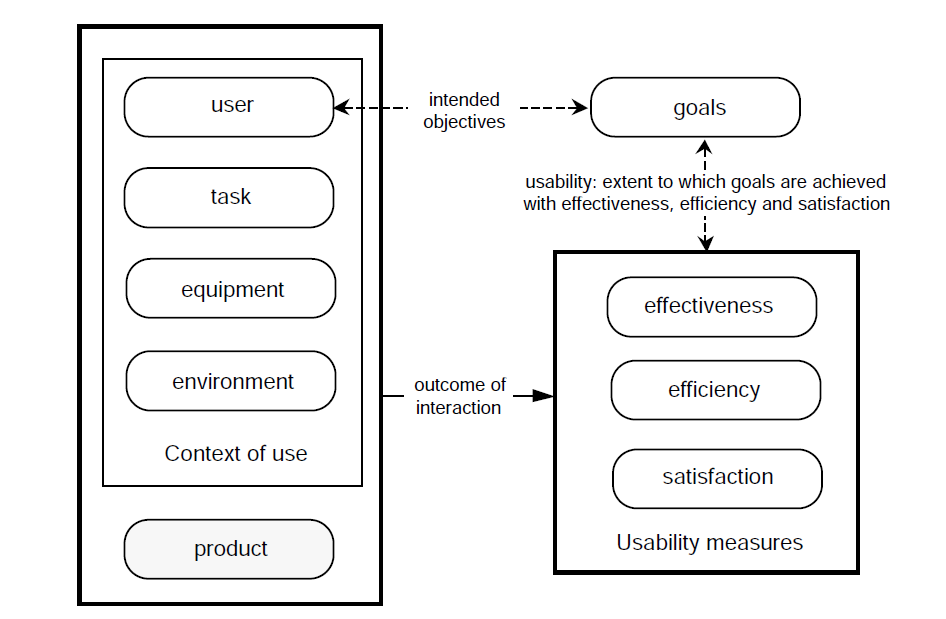
\includegraphics[scale=0.285]{img/usability1.png}
\end{figure} 

ISO 9241-11 describes how the usability of a product can be defined, documented and
verified as part of a quality system which conforms to ISO 9001 (Figure \ref{fig:usability2}). The overall context of use should be identified, usability requirements should be specified, usability issues should be monitored during development, and the usability achieved should be evaluated. \\
Dealing with usability as part of a quality system for design and development of products, as specified in ISO 9001, involves the systematic identification of requirements for usability, including usability measures and verifiable descriptions of the context of use. These provide design targets which can be the basis for verification of the resulting design. ISO 9001 specifies what is required for a quality system. A quality system is a documented set of procedures intended to ensure that a product will meet initially stated requirements. A quality system is a desirable (though not sufficient) condition for achieving the quality of the end product. 

\begin{figure}[H]
\caption{Quality Plan. Source: \cite{bevan1995human}}
\label{fig:usability2}
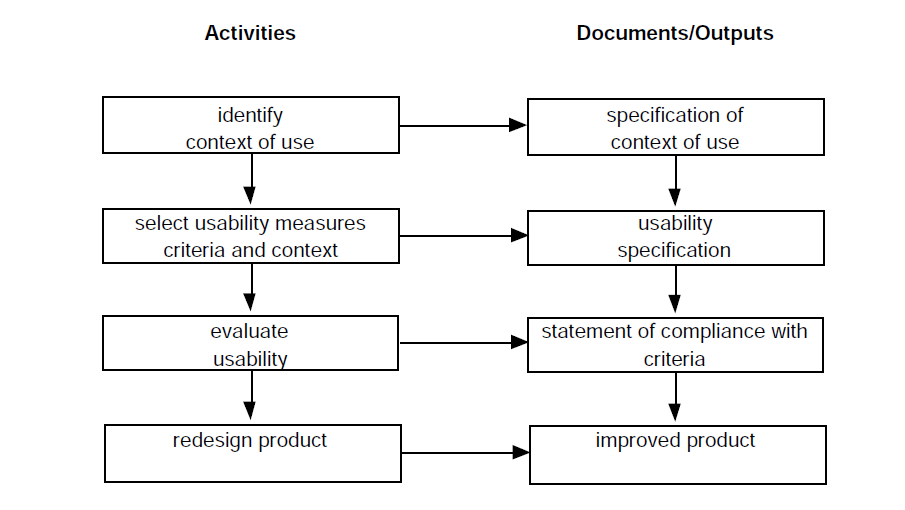
\includegraphics[scale=0.3]{img/usability2.png}
\end{figure} 

\textbf{Usability requirements:} Prior to the development of a custom system, the purchasing
organisation should specify the usability requirements which the system must meet and
against which acceptance testing may be carried out. Specific contexts in which usability is to
be measured should be identified, measures of effectiveness, efficiency and satisfaction
selected, and acceptance criteria based on these measures established. \\
\textbf{Monitor usability:} At various stages during the development process the developer should
measure the usability achieved against these targets. This information enables objective
decisions to be taken about the need for design changes to enhance usability, and about trade-offs
which may be appropriate between usability and other requirements. \\
\textbf{Usability evaluation:} The characteristics of the context in which a product is likely to be
used need to be identified. To ensure the validity of test results the users, tasks and
environments used for the evaluation should match the real context of use as closely as
possible.


\section{Framework for Usable Security}
In the previous section, usability was explained as a broad concept. It is applicable to any system which is directly interfaced by a user or has an impact on user perforamnce. In this section, we specialize the usability concept to security in virtual power plants and as will further be explained, to authentication mechanisms.\\ Since, usability and security are normally at opposite ends of the spectrum, there are no uniform set of criteria or guidelines that define a usable security system. Nurse et al\cite{nurse2011guidelines} compiled a list as guidelines for usable security.
\newline
To design a security system that is usable, we need appropriate metrics to measure its performance, especially in context of virtual power plants. Therefore, we need to define such metrics. With the security system in focus, the usability metrics must stem from the properties of security themselves. Since the security system is designed for virtual power plants, some factors are automatically constrained. Due to the volatile nature of power plants, time is of utmost importance. Hence, a time efficient system is a requirement. We also need to consider the performance of the operator under stress. A well designed system reduces operator responsibilities like memory use for passwords and encourages productivity. Through this process, we then develop a security with a view of usability in the design stage itself, rather than first building a security system and then attempting to incorporate usability. When designing a security system, each interface of security could be tested for its usability wherever applicable. A less usable component may affect usability of another. The issue at hand is that due to the lack of usability metrics or any quantifiable value, any system cannot yet be defined as usable or unusable. \\


Quality in Use Integrated Measurement(QUIM)\cite{seffah2001quim} was proposed to primarily address these issues by aggregating usability standards, metrics and methods from numerous sources in one centralized knowledge base. QUIM is a repository of 10 factors, 26 criteria, and 128 metrics for assessing usability/quality in use of software systems. Most of the existing usability models/standards may be seen as specific instances of the QUIM model. \\

Usability of a system, though determined by efficiency, effectiveness and satisfaction, is still not quantified. Furthermore, the three factors can be measured in various ways for different systems. To measure these factors, a relation between security and usability must be established. In the presence of such a relation, a security system's properties can be optimized, via metrics, such that usability properties are satisfied. \textit{This method can be used to integrate usability into any system instead of security systems.} In essence, each property has a metric with a desirable value that makes the system usable. A security system will have to go through a usability engineering cycle subject to constraints and metrics. To achieve strong security, security engineering must begin parallel to system development, which is known as security-by-design. Similarly, usability must be considered in the design phase as well. Individual components may be evaluated for usability. This may be considered as \textbf{Usable Security by Design.}


\subsection{Deriving Usability for Authentication}
With respect to the virtual power plants, the asset we are trying to protect is the control and information flow of the grid. Therefore, being a critical infrastructure, their estimated value is evidently high.   
\newline The countermeasure, in this case, is an authentication system. To move forward with the framework, we need to identify the elements of the authentication system. Generally, they contain: An interface, a database, an authentication protocol run, key/token management and encryption algorithms. All the elements of the system can be measured using suitable metrics to quantify their impact on the usability of the system. In table \ref{tab:security-usability-relation}, different properties or factors affecting security are listed. The third column contains these factors, the second column contains the criteria for usability, which also represent the requirements for usability in this case and the first column contains the properties and factors affecting usability. The table is arranged such that if the security factors are optimized, they either directly satisfy the usability factors(or properties) in the first column or they satisfy the usability criteria(in the second column) and transitively satisfying the usability factors(or properties). 


\begin{center}
\begin{table*}
\caption{Relation between security and usability}
\label{tab:security-usability-relation}
\resizebox{14cm}{!}{
\begin{tabular}{|c|c|c|} 
\hline
\multicolumn{2}{| c |}{\textbf{Usability}}
& \textbf{Security} \\
\hline
\textbf{Factors and Properties} & \textbf{Criteria/Requirements} & \textbf{Factors and Properties} \\
\hline
Effectiveness & Accuracy & EER, Accuracy \\
\hline
Efficiency & Minimal Action & \makecell{Task Completion Time, \\ Monetary cost of performing the task} \\
\hline
{Satisfaction} & {Operability, Minimal Action} &  {Interface Design} \\
\hline
Productivity & Memory Load & Authentication Token \\
\hline
Learnability & \makecell{Time to learn functionalities,\\ Minimal Action} &  Interface Design \\
\hline
\end{tabular}
}
\end{table*}
\end{center}


The second column in table \ref{tab:security-usability-relation} specifies the requirements(or criteria) for usability of a security system. These criteria were specifically selected for a scenario involving a user attempting to gain access through an authentication mechanism. These requirements need to be quantified with metrics for an evaluation. the table \ref{tab:possible-values} shows the metrics and the desired values for this specific use case. In power plants, it is undesirable to lock the operator out of the system. Therefore we need a highly accurate and efficient system, hence an accuracy as close as possible to 100\% and an EER, in case of biometric systems, as low as possible is desirable. We do not want the operator to be stressed while waiting for authentication, hence a fast system is needed. Both Interface Design and Memory Load can be rated by the operator based on scale from 1 to 5, where 1 is "Very Uncomfortable" and 5 is "Very Comfortable". The operator must be comfortable with using the system and must also not expend too much memory to prevent stress. Both metrics should be placed 4 or more.

\begin{center}
\begin{table}
\caption{Possible values for metrics}
\label{tab:possible-values}
\resizebox{9cm}{!}{
\begin{tabular}{|c|c|}
\hline
\textbf{Security Metric} & \textbf{Permissible Range} \\
\hline
EER & \textasciitilde 0\%\\
\hline
Accuracy  & \textasciitilde 100\%. \\
\hline
Task Completion Time &  8-10 seconds \\
\hline
Interface Design & >4\\
\hline
Memory Load & >4\\
\hline
\end{tabular}
}
\end{table}
\end{center}

Therefore, a \textit{usable security framework for an authentication system} consists of an authentication system which includes a user-friendly interface, requires a user to have minimalistic or easy to use authentication tokens, satisfies the criteria for a conventional security system such as Confidentiality, Integrity and Availability in addition to all the usability factors mentioned in \ref{tab:security-usability-relation}. The evaluation of these factors via usability criteria with respect to their metrics should fall in the permissible zone. The operator also must provide feedback and specify the drawbacks, if any and suggestions to improve the system from the perspective of usability. \\
The factors mentioned in the third column are specific to authentication mechanisms. If usability was being considered for any other system, the respective factors would be derived and placed accordingly in that column. For example, consider an organization attempting to develop self-driving automobiles. User experience plays a big part in such an inventive technology. To measure usability of such vehicles, effectiveness will be determined by the performance of the vehicle. It is up to the discretion of the organization to determine which metric they would prefer to use to measure the performance. An example could be speed or acceleration. Efficiency can be measured by fuel consumption. Satisfaction can be measured by user feedback. In this way, the framework could be used for any system.

\subsection{Using The Framework}
To apply the usable security framework, the organization intending to use it has to specify the goals on the system. Similar systems may be optimized in different ways, hence the developers need to specify their priorities based on context of use. The important factors and properties affecting the system must be listed and with respect to the priorities, i.e, goals of the system and the developers, those factors affecting the user most should be selected. For example, let the goal be a highly user-friendly yet efficient authentication mechanism for power plant. Therefore, Interface Design and Time as a resource are goals and are priorities.\\
The usability framework, with the help of QUIM, breaks down usability factors into criteria that can be quantified. Those usability factors that are of importance to the developers must be focused upon, however, the three usability factors, efficiency, effectiveness and satisfaction must all be used to satisfy usability, as per ISO 9241-11. In our example, task completion time and memory load will be the focus and hence it will need to be optimized.\\
In the next step, those factors derived from the target system must be used as quantifiable values to measure the criteria specified in table \ref{tab:security-usability-relation}. If a criteria cannot be quantified, alternative criteria can be selected from the QUIM usability criteria. In any case, the prioritized factors must be quantified. In our example, accuracy is a measurable quantity of the system as well as the usability criteria used to determine the efficiency.\\
Accordingly, the factors measured from the system must be used to quantify the usability criteria, which help measure the usability factors. 

\subsection{Validation of the framework}
To demonstrate how this framework could be used, we use an example. Two different authentication systems were tested, a fingerprint matching system and a simple password system. The evaluation involved participants using both types of systems and then answering a questionnaire. To assess fingerprint matching, two approaches were used. Since there are several types of fingerprint matching algorithms, performance may vary. Therefore, the most common implementations found in real life were used. First, an optical scanner of fingerprints was evaluated. An optical scanner scans the fingerprint into an optical image and compares the image as is with a database of images. This process is slow and less secure, as images of fingerprints are stored unprotected in the database. The second kind was a capacitive scanner, where fingerprints are read using varying electric charges when a ridge comes in contact with the scanner. This change is charge is converted to digital data, which is then analysed to look for unique features. Data is stored digitally, though not necessarily encrypted. This form of storing data is still vulnerable but more secure than images. There were 30 participants whose fingerprints were added to a database of more than 1000 entries. The results of the capacitive scanner were found to be more optimal. They are shown below:

\begin{center}
\begin{table}[H]
\caption{Results for Biometric systems.}
\label{tab:result1}
\resizebox{9cm}{!}{
\begin{tabular}{|c|c|}
\hline
\textbf{Security Metric} & \textbf{Observed values} \\
\hline
EER & 3.9\%\\
\hline
Accuracy & 96.1\%. \\
\hline
Task Completion Time & Average of 1.8 seconds \\
\hline
Interface Design & 4.2\\
\hline
Memory Load & 5\\
\hline
\end{tabular}
}
\end{table}
\end{center}

The EER and Accuracy values claimed were 1.9\% and 98.1\% respectively by the algorithm. The fingerprint matching was not developed in-house but was rather off the shelf for assessment. Possible reason for the lower values is the smaller sample space. The values shown against "Interface Design" and "Memory Load" are mean values of the scores given by participants. The scores were based on a scale from 1 to 5, where 1 represents "Very Uncomfortable" to "Very Comfortable".\\
Shown below is the inference table for password systems. Typical password systems include the user presenting a username and password, both entered by the user. The same setup was used for the following evaluation. Users were registered with a simple password system and then were asked to login. Standard password recommendations were used, such as using passphrases, combinations of letters, both uppercase and lowercase, numbers and symbols. 

\begin{center}
\begin{table}[H]
\caption{Results for password based systems.}
\label{tab:result2}
\resizebox{9cm}{!}{
\begin{tabular}{|c|c|c|}
\hline
\textbf{Security Metric} & \textbf{Observed values} \\
\hline
Accuracy & 100\%. \\
\hline
Task Completion Time & Avg of 12.2 seconds \\
\hline
Interface Design & 4.7\\
\hline
Memory Load & 3.5\\
\hline
\end{tabular}
}
\end{table}
\end{center}

Interface Design and Memory Load were scored with the same method as for biometric systems. Interface design received a higher score due to the familiarity to users, however due to complicated passwords, it was harder to remember multiple difficult and complex passwords for various systems simultaneously. It also affected the task completion time, which was relatively longer. Accuracy is 100\% since a correctly entered password was never rejected. We are not counting mistyped passwords. A reason for using accuracy is that the measure used for biometrics is accuracy. In biometric systems fingerprints are rarely falsely entered, although a possibility. Users are aware of which fingerprint is required. Therefore, in fingerprint systems accuracy of the algorithm is used as a measure for the performance. To keep the consistency, accuracy was used for password systems, even though accuracy is normally not a measure for such systems. A correctly entered password will never be rejected, provided the credentials exist and are legitimate.

\subsection{Inference}
Now that we have results of two different authentication systems, a comparison can be made to assess which is more usable of the two. Tables \ref{tab:result1} and \ref{tab:result2} can be compared now that they have normalized metrics, i.e, common metrics. Since the EER is only used in biometric cases, it will not be used for comparison. Password based systems have a 100\% accuracy and a high rating for "Interface Design", but as explained earlier, these values were expected. Accuracy of biometric system observed as 96.1\% is still formidable. In case of a false negative, the task completion time, being exceptionally low, compensates for the time lost. The key factors are Task Completion Time, Interface Design and Memory Load. The fingerprint matching system used was exceptionally fast at 1.8 seconds for a successful authentication, although this can be attributed to relatively low sample space and the use of a capacitive scanner. In contrast a password system took an average of 12.2 seconds. This may be due to complexity of passwords, typing speed and additional time required to enter the user identifier such as a username. Interface design were both scored above 4, with password systems higher due to its familiarity to users. Memory Load, being a very important focus, due to difficulty in remembering difficult passwords especially under stress, shows that password systems are not preferable at all. Fingerprint systems require no memory use and are very usable.\\
It can be seen from the comparison that biometric systems such as fingerprint recognition and matching systems are accurate, faster, easy-to-use and are hence very usable.\\
A conclusion drawn from the analysis is that there can be no standard values for a usable system, i.e, one set of values for the usability factors cannot be applied to all systems. Usability values are subjective to the system and to the goals of the organization. It could be possible to set a threshold for a specific type of system. For example, several single factor authentication systems could be tested. The system that is determined to be the most usable may have its values set as a threshold for usable authentication mechanisms. However, these values of the framework can only be applied to single factor authentication mechanisms and no other system. This could be extended to two factor authentication mechanisms and other systems as well.

\section{Example Use Case}
To describe the approach for usability-by-design, or in this case usable security-by-design, the use case of DER scheduling in Dynamic Virtual Power Plants was used. The figure \ref{fig:uml_diag} depicts a UML diagram of a typical scheduling process that takes place in Dynamic Virtual Power Plants\cite{niesse2014conjoint}. The distributed agents in the field are responsible for scheduling based on information such as predicted energy generation from its Distributed Energy Resource(DER), Market information, available agents in the area etc. and forms a coalition of energy sources to meet the energy demand.

\begin{figure}[H]

\caption{UML diagram of rescheduling process.}
\label{fig:uml_diag}
\begin{sequencediagram}

\def\unitfactor{0.4}
\newthread{a}{VPP SP}
\newinst[2]{b}{IED(all)}
%\newinst[2]{c}{Metering}
\newinst[2]{d}{DER}

\begin{call}{b}{Req\_Markt()}{a}{Markt\_Info}
\end{call}

\begin{call}{b}{Req\_Agent\_List()}{a}{Agent\_Info}
\end{call}

\begin{callself}{b}{Coalition and Scheduling}{}
\end{callself}

\begin{call}{b}{Set\_point()}{d}{ACK}
\end{call}{ACK}

\begin{call}{b}{Reschedule()}{b}{}
\end{call}

\begin{call}{d}{Metering Data}{b}{}
\end{call}

\begin{call}{b}{Reschedule()}{b}{}
\end{call}

\end{sequencediagram}
\end{figure}


Employing the method in Uslar et. al\cite{uslar2014security}, the mapping shown in figure \ref{fig:HLdiag} is obtained using the NIST 7628 logical reference diagram\cite{NIST7628:2014}. There are 4 identified actors and their respective logical interfaces. The actor "1 Plant Control System" corresponds to the DER at the generation side, "46 Transmission IED" is the field agent on an Intelligent Electronic Device(IED) as described in Dynamic Virtual Power Plants, "30 Energy Management System" is an actor within the operation domain which corresponds to the Virtual Power Plant Service Provider interface between the system and the IED. All communication takes place through the "37 Transmission SCADA". Each actor is interfaced with Transmission SCADA as it is the actor that represents the transmission in a power system. Each interface has a set of specific security requirements described in NIST 7628. 

\tikzstyle{decision} = [diamond, draw, fill=blue!20, 
    text width=2.25em, text badly centered, node distance=1.5cm, inner sep=0pt]
\tikzstyle{block} = [rectangle, draw, fill=blue!20, 
    text width=5em, text centered, rounded corners, minimum height=2em]
\tikzstyle{line} = [draw, -latex']
\tikzstyle{cloud} = [draw, ellipse,fill=red!20, node distance=1.5cm,
    minimum height=1em]
\definecolor{carnationpink}{rgb}{1.0, 0.65, 0.79}
\begin{figure}[H]
\caption{High Level Diagram for the Interfaces.}
 \label{fig:HLdiag}
\begin{tikzpicture}[scale=0.1, node distance = 3cm, auto]
	\definecolor{aqua}{rgb}{0.0, 1.0, 1.0}
	\definecolor{aureolin}{rgb}{0.99, 0.93, 0.0}
	\definecolor{carnationpink}{rgb}{1.0, 0.65, 0.79}
    % Place nodes
   	\node [block, line width=1mm, fill=carnationpink] (PCS) {1 Plant Control System}; 
    \node [block, fill=aureolin,right of=PCS] (SCADA) {37 Transmission SCADA};
    \node [block, fill=aqua,right of=SCADA] (IED) {46 Transmission IED};
    %\node [block, fill=aureolin,below of=IED] (SCADA1) {37 Transmission SCADA};
    \node [block, fill=aureolin,below of=SCADA] (EMS) {30 Energy Management System};
    % Draw edges
    \path [line] (PCS) -- node{U80}(SCADA);
    \path [line] (SCADA) -- node{U81}(IED);
    \path [line] (SCADA) -- node{U83}(EMS);
   	\draw[green,thick,dashed] ($(PCS.north west)+(-0.3,0.6)$)  rectangle ($(SCADA.south east)+(0.5,-0.6)$) node [pos=0]{Interface Category 1};
   	\draw[blue,thick,dashed] ($(SCADA.north west)+(-0.5,1.0)$)  rectangle ($(IED.south east)+(0.3,-1)$) node [ below left]{Interface Category 3}; 
   	   	\draw[red,thick,dashed] ($(SCADA.north west)+(-0.3,0.8)$)  rectangle ($(EMS.south east)+(0.8,-0.8)$) node [pos=0]{Interface Category 6}; 
\end{tikzpicture}
\end{figure}

Since there may be several interfaces with common requirements, NIST 7628 categorizes interfaces into categories with similar requirements. For example, interface U83 falls under category 1. Under category 1, security requirements such as AC-14, IA-4, IA-6 and so on are specified. AC-14, for example, is a requirement that allows certain actions, under certain circumstance such as emergencies, to be performed without identification and authentication of the operator. Such a requirement can actually be exploited by a malicious outsider or an attacker. An attacker may simply induce an attack or a false alarm, in which case security mechanisms such as authentication procedures will be suspended. The attacker then has free access to the system with the authentication procedure bypassed. It is understandable that such a requirement is recommended, in order to prevent the operator from being locked out of the system during emergencies. However, it clearly has flaws which can be exploited. A suitable solution for this flaw is the introduction of an usable authentication mechanism that secures the system access as well as reduces the burden of authentication on the operator by its usability.\\

A usable authentication mechanism can be developed to aid the operators of power plants. Developing such a mechanism requires user preferences prior to its implementation. A survey can be conducted to obtain the opinions and preferences of grid operators. This survey will have to conducted early, i.e, prior to the requirement specification. More detail on the method to integrate usability into the software development lifecycle is described in the following subsection.



\subsection{Integration into Security Development Lifecycle}
An important aspect of usability engineering is that usability must be considered early on in software product development lifecycle. Usability of a product or a system can be measured after its development but cannot be integrated thereafter. To ensure the usability of product is as required, it must be considered early on. Each product has a set of target users and their preferences must be considered before product design. \\
Microsoft has developed a Security Development Lifecycle\cite{howard2006security}, which we shall use to define where and when to use the usability framework. This lifecycle was developed to produce more secure software, and is step towards security-by-design. The Security Development Lifecycle Process is divided into several phases which are further divided into stages:
\begin{itemize}
\item Training: Known as phase 0, where developers are informed about security basics and recent trends in security and privacy. In this phase, developers must obtain information about preferences from the target user group. This information contains preferences about kind of system which could be used, willingness to learn a new system, trustfulness in an existing system, comfort in using an existing system and resources they are willing to expend to achieve their goal. An example is how time they willing to spend to accomplish the task the security system is required to complete. The framework may be used to set specific goals. Additionally, certain usability factors may be given priority based on goals of the system, such as efficiency, i.e, the amount of resources utilized to achieve the goal of the system must be limited and hence must not cross a specified limit.

\item Requirements: Based on user preferences, the developers can narrow down the possibilities of implementation. Preferences may not necessarily be unanimous, in which case the developers and users must come to an agreement for the most preferable options. Developers may brainstorm best available technology required for the narrow possibilities of implementation to meet the specified goal. Security requirements take precedence over usability requirements. Therefore, first the security goals can be used to filter the implementation possibilities followed by the usability goals.

\item Design: The focus of this phase is threat modelling and attack surface analysis, hence it is in the best interest to focus on security goals in this phase. After analysing security, the model may be used to assess if the performance goals affecting usability are met, such as accuracy and task completion time.

\item Implementation: Based on requirements and design method selected, the developers can engineer a system that is secure and usable. The team of engineers follow the conventional software development process including coding, testing and integration.  Steps are taken to remove security flaws. Security takes precedences over usability once more. 

\item Verification: The system undergoes testing and the team conducts a "security push" that includes security code reviews targeting the finished version of the software. This is to ensure the final product meets the security goals and a deeper review of the system. A usability review may follow the security review to ensure the usability goals have been met.

\item Release: This phase is intended to give the developer team and the organization the big picture of the security software and its ability to withstand attacks. If vulnerabilities are found, they need to be fixed. Usability aspects of the product may be beta tested by a user from outside of the team.

\item Response: Any vulnerabilities found post release will be patched in the response phase. This is largely achieved by updates. Detection of vulnerabilities also help eliminate further vulnerabilities before they are discovered. Usability concerns may be reported, however cannot be improved without large scale replacements incurring high costs. The concerns may be taken into consideration for the next product cycle.
\end{itemize} 



\section{Conclusion and Future Work}
Extensive security measures will be needed to protect power plants and other critical infrastructures from various kinds of attacks. In order to aid the operator in attack scenarios, the system in place should be usable. To assess usability of systems, a usability framework for security was derived, which helps establish the relation between the target system, in this case, security and usability.  With the use of this framework, it is possible to compare multiple systems and determine if they are usable or not. This was demonstrated by comparing two systems used in authentication mechanisms, a password based system and a fingerprint matching system. It is important to note that this framework can applied subjective to the system and the mechanism. Different systems will have different values for the framework and different systems factors may be related to usability criteria and factors. The framework paves the way to \textit{usable security by design}. Future Work will involve defining detailed metrics with methods or formulae to measure them. Metrics may also be defined to determine the degree of performance of a user under various scenarios. Specific usability frameworks for various systems may also be derived.

